
\section{Auswertung}
\label{sec:Auswertung}
\subsection{Überprufung des Laserbetrieb}
\label{sec:über1}
In den Abbildungen (\ref{fig:mess1}) und (\ref{fig:mess2}) sind die beiden aufgenommenen Bilder zu sehen, die Speckle sind deutlich sichtbar. Der Schwellenstrom beträgt in etwa $I=\SI{40}{\milli\ampere}$
\begin{figure}[h!]
  \centering
  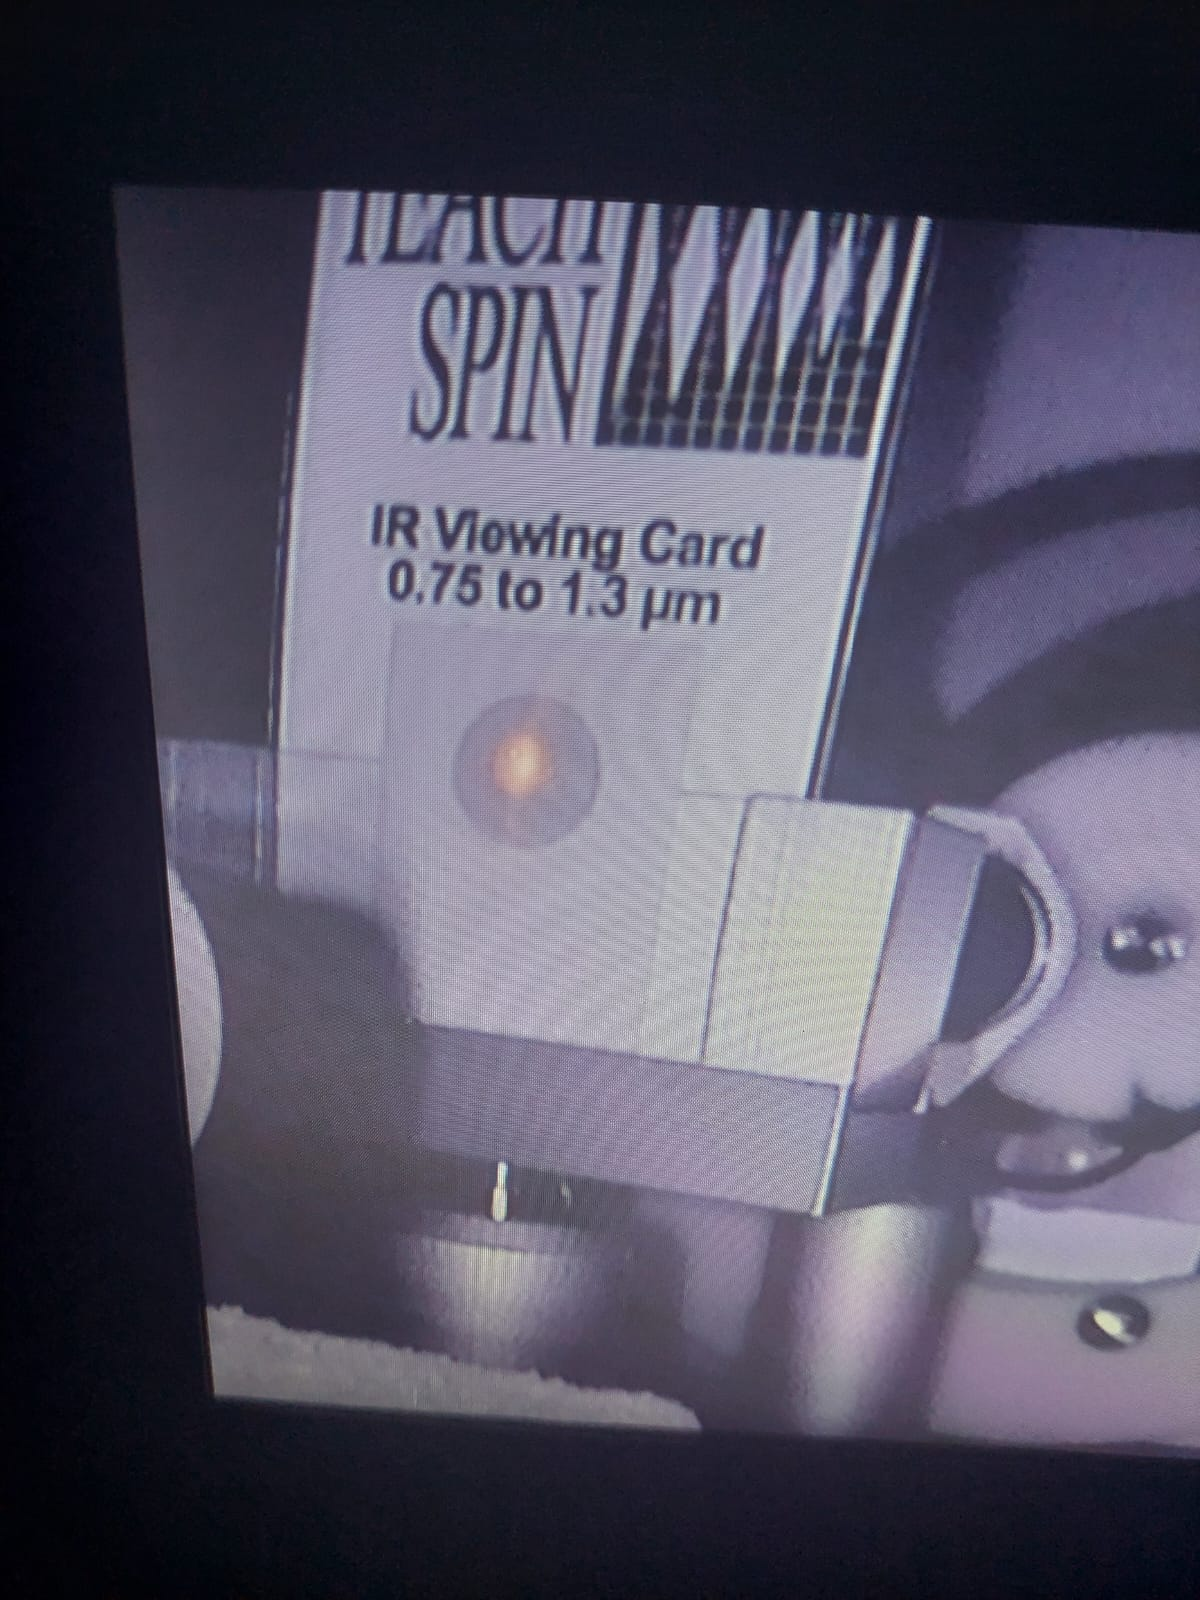
\includegraphics[scale=0.1]{fig/led.jpeg}
  \caption{Laserdiode im LED-Betrieb.}
  \label{fig:mess1}
\end{figure}
\FloatBarrier
\begin{figure}[h!]
  \centering
  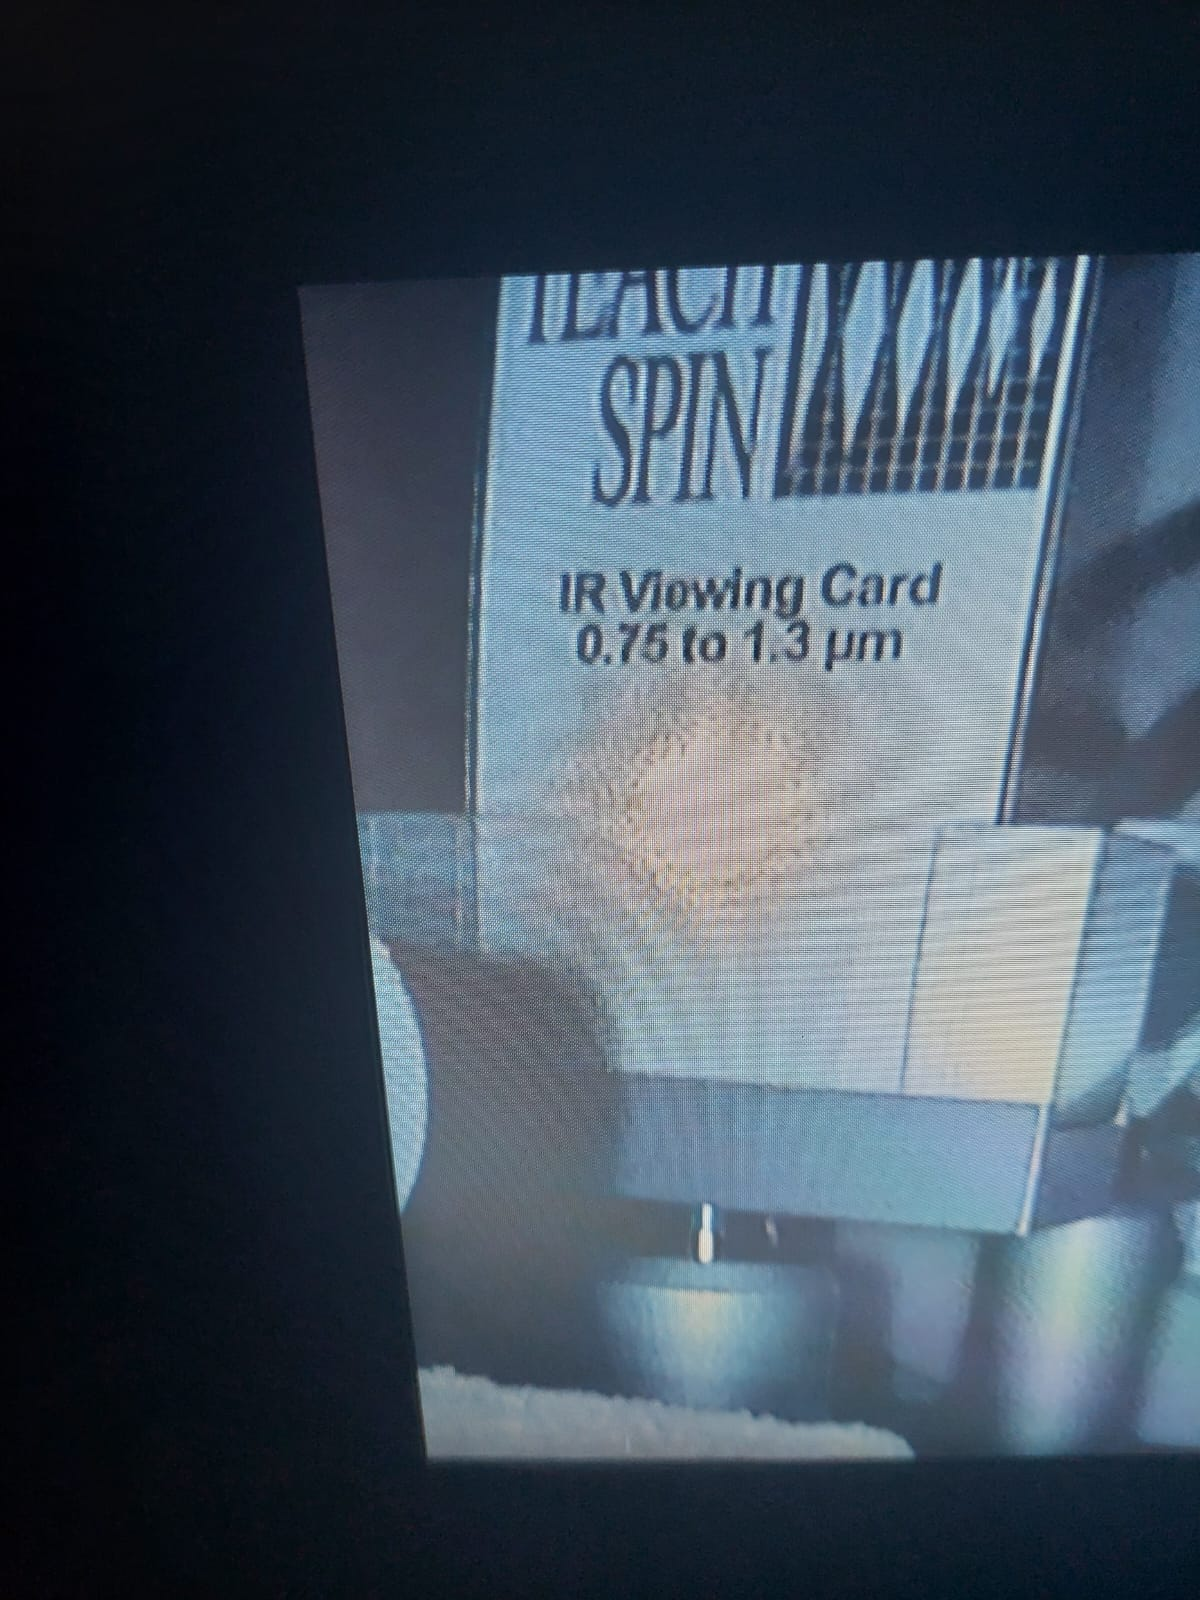
\includegraphics[scale=0.1]{fig/laser.jpeg}
  \caption{Laserdiode im Laserbetrieb.}
  \label{fig:mess2}
\end{figure}
\FloatBarrier
\subsection{Bestimmung der Absorptionswellenlänge}
\label{sec:über2}
In Abbildung (\ref{fig:mess3}) ist das aufgenommene Bild zur Bestimmung der Absorptionswellenlänge zu sehen.
\begin{figure}[h!]
  \centering
  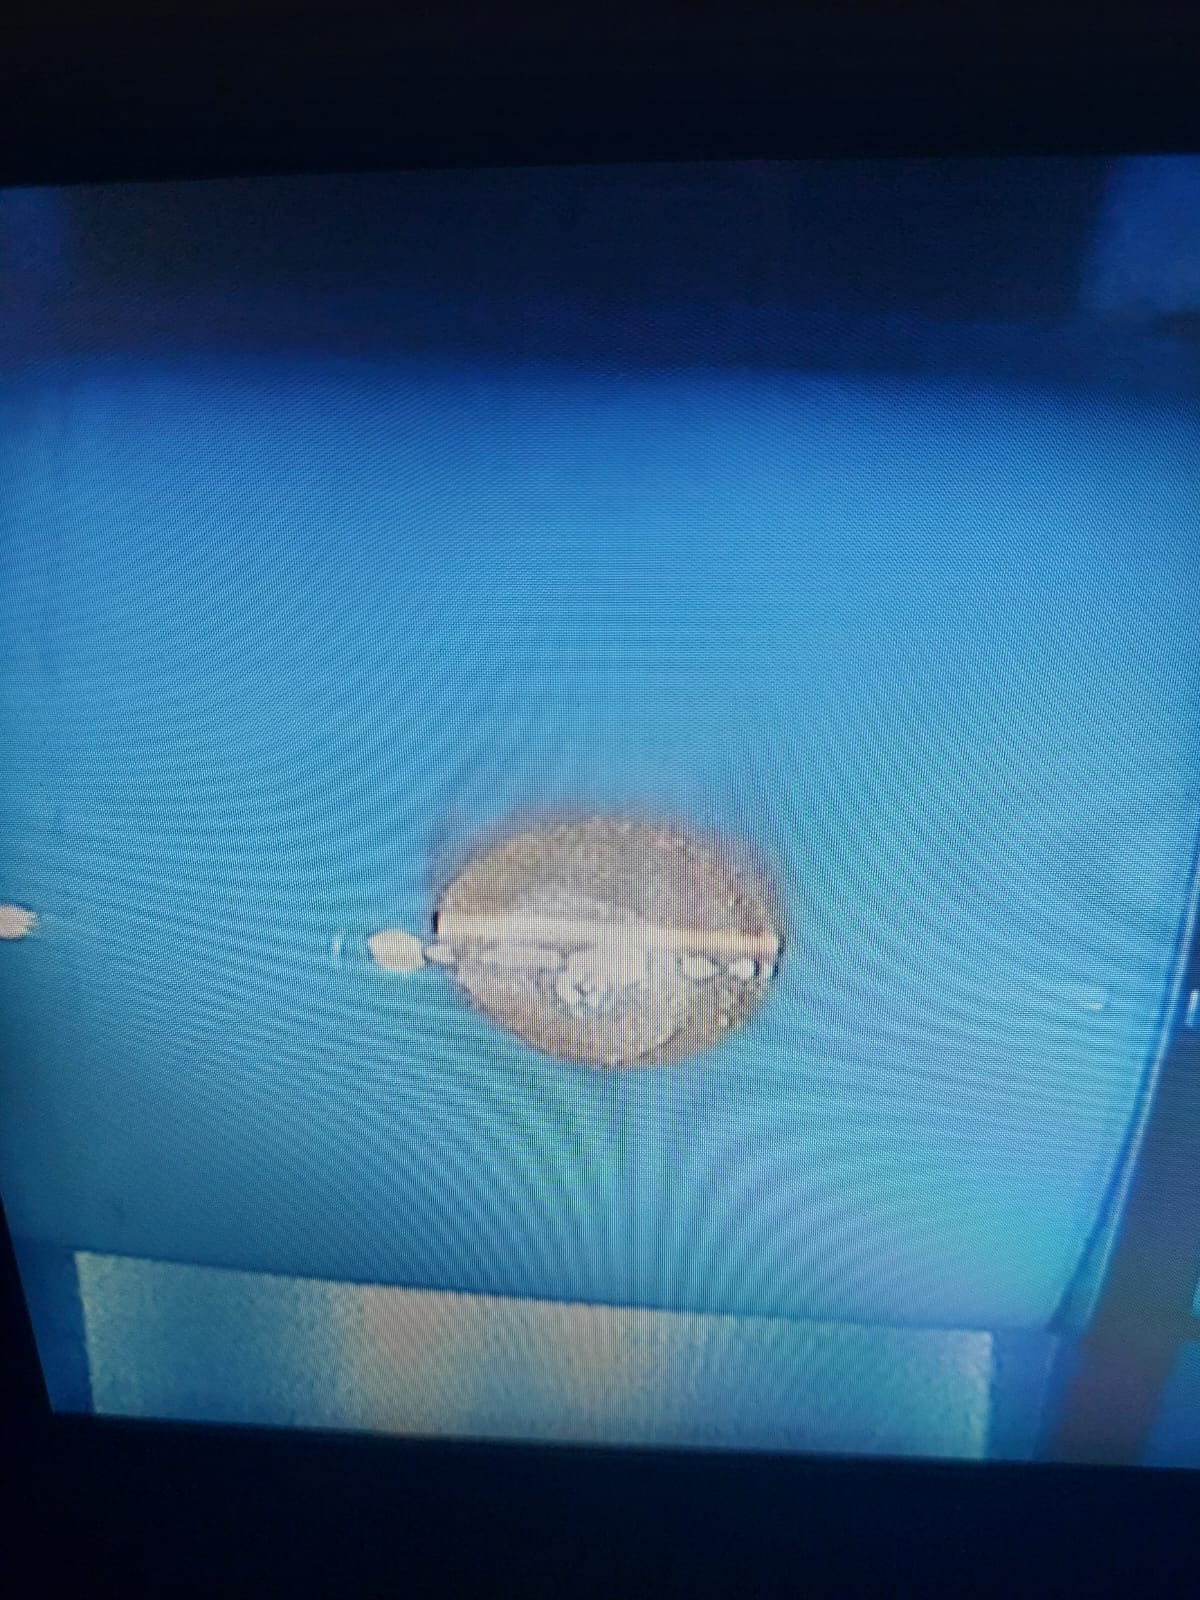
\includegraphics[scale=0.1]{fig/fluor.jpeg}
  \caption{Bild der Rubidiumzelle.}
  \label{fig:mess3}
\end{figure}
\FloatBarrier
\subsection{Bestimmung des Absorptionsspektrum}
In Abbildung (\ref{fig:mess4}) ist das aufgenommene Absorptionsspektrum zu sehen.
\begin{figure}[h!]
  \centering
  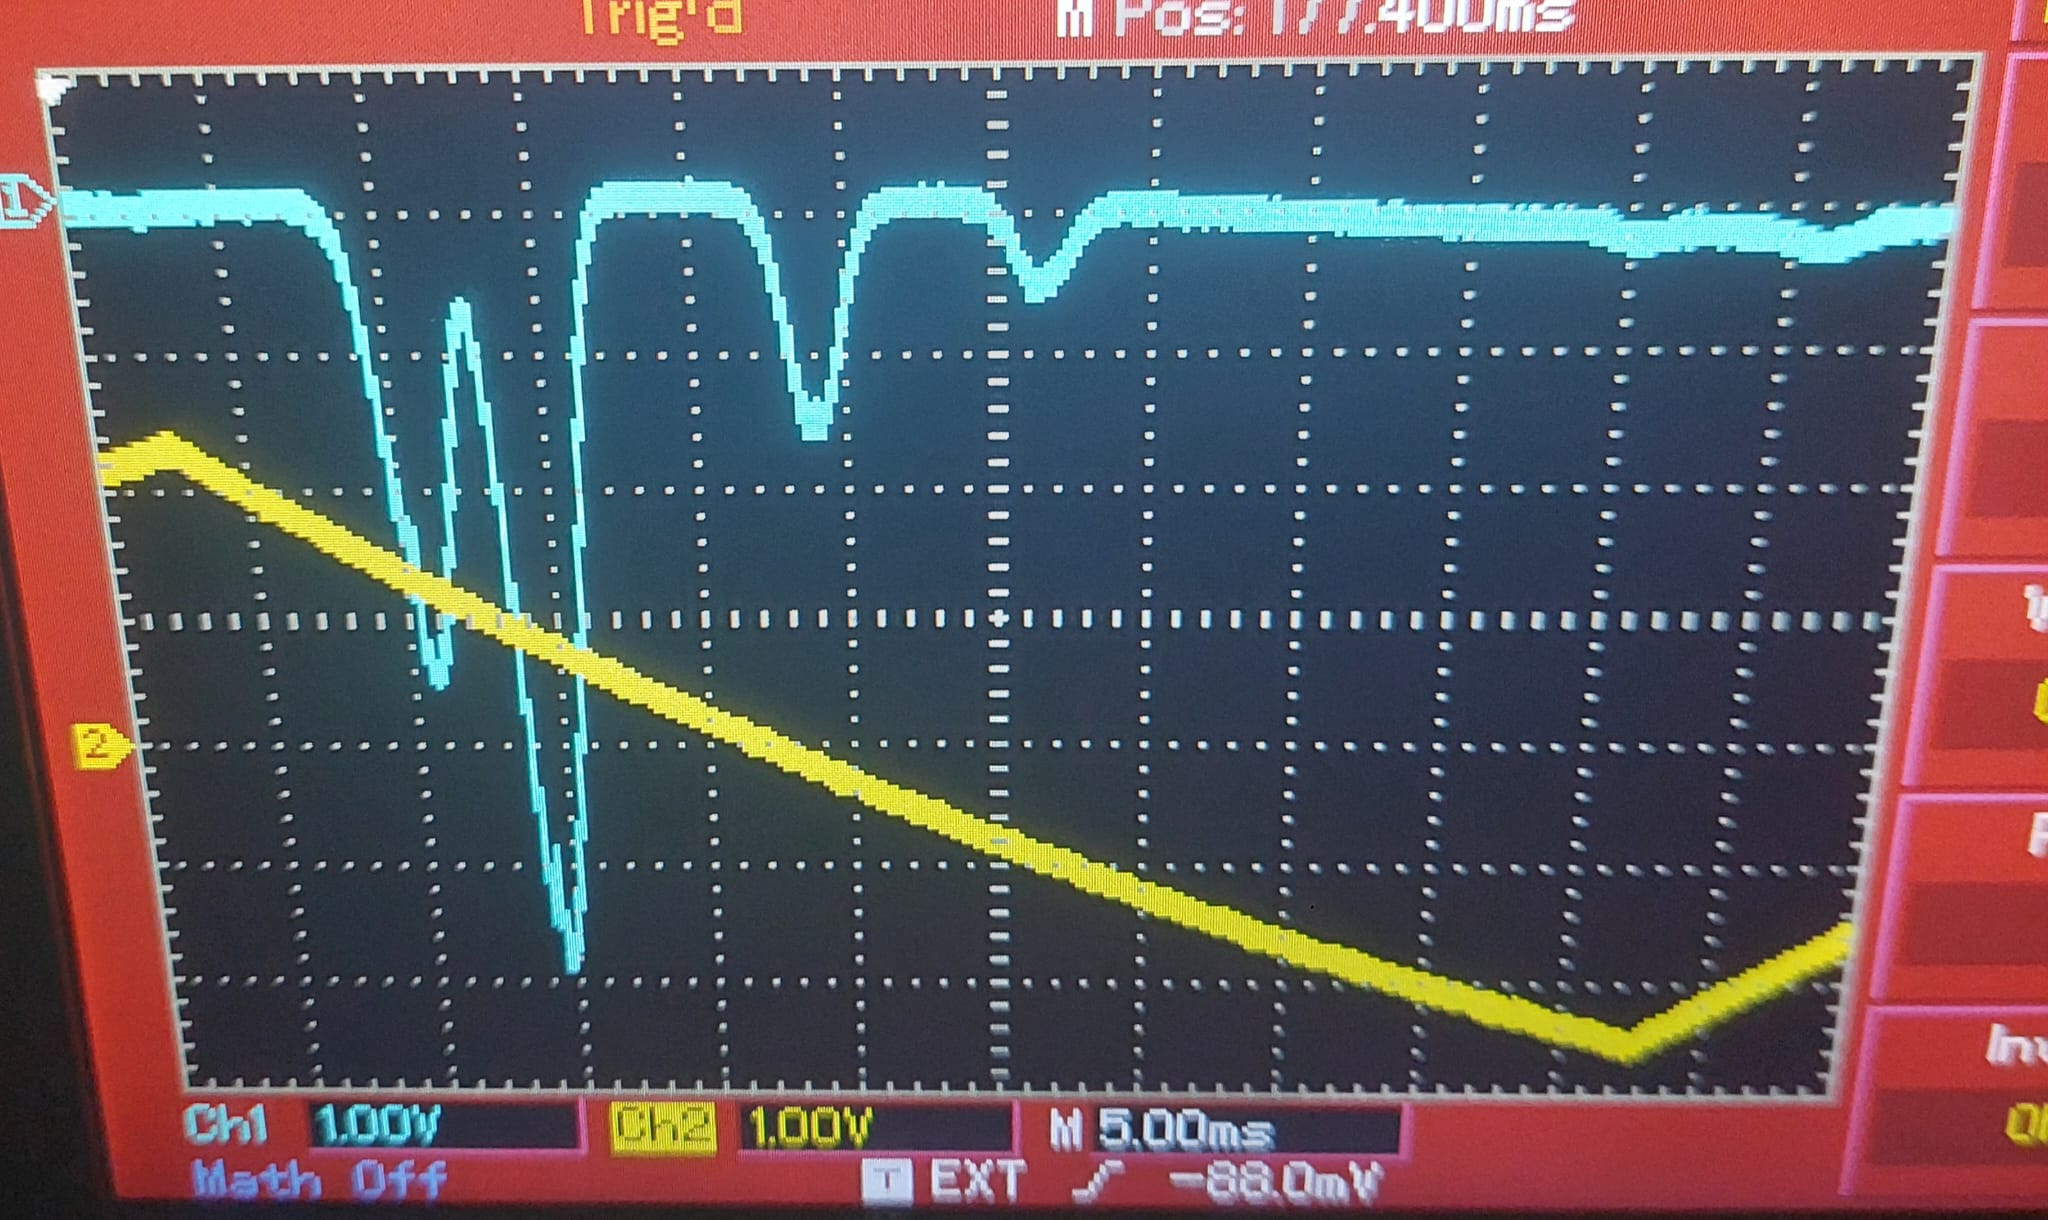
\includegraphics[scale=0.15]{fig/spektrum.jpeg}
  \caption{Absorptionsspektrum des Rubidium.}
  \label{fig:mess4}
\end{figure}



%\begin{figure}[h!]
%  \centering
%  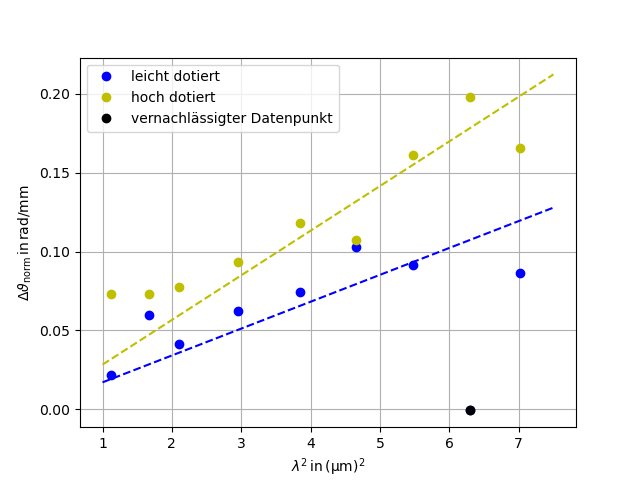
\includegraphics[scale=0.7]{fig/deltaTheta.png}
%  \caption{Grafische Darstellung der Messdaten aus den Tabellen \ref{tab:tief} und \ref{tab:hoch}.}
%  \label{abb:delta}
%\end{figure}
